\documentclass[preprint]{elsarticle}

% layout
\usepackage{hyperref}
\usepackage{geometry}
\geometry{a4paper,left=40mm, right=40mm, top=30mm}
\bibliographystyle{model5-names}\biboptions{authoryear}
\usepackage{multicol}
\usepackage{url}

% footer
\makeatletter
\def\ps@pprintTitle{%
 \let\@oddhead\@empty
 \let\@evenhead\@empty
 \def\@oddfoot{\centerline{Preprint \textemdash \: \today}}%
 \let\@evenfoot\@oddfoot}
\makeatother

% text & symbols
\usepackage{csquotes} \usepackage{amsmath} \usepackage{amssymb}
\usepackage[official]{eurosym} \usepackage{bm} \usepackage{bbm}
\newcommand{\ah}[1]{{\bf[AH: }#1{\bf]}}
\newcommand{\ag}[1]{{\bf[AG: }#1{\bf]}}

% figures & references
\usepackage{graphicx} \graphicspath{{../figs/}}




\begin{document}






\noindent \textbf{Documentation}
\section{Overview}

\begin{table}
  \centering
  \small
\begin{tabular}{r p{4.0cm}}
  Term & Description \\ \hline
  \multicolumn{2}{l}{\textbf{Indices}} \\
  $i$ & Generation technology \\
  $r$ , $r'$ & Region \\
  $t$ & Time step \\
  \multicolumn{2}{l}{\textbf{Sets}} \\
  $\mathcal{I}$ & Technologies: baseload ($b$), peaking ($p$), wind ($w$), solar ($s$), unmet demand ($u$) \\
  $\mathcal{D}$ & Decision variables \\
  \multicolumn{2}{l}{\textbf{Parameters}} \\
  $C_{i}^\text{gen}$ & Install cost, technology $i$ (\pounds m/GWyr)\\
  $C_{r, r'}^\text{tr}$ & Install cost, transmission, region $r$ to $r'$ (\pounds m/GWyr) \\
  $F_{i}^\text{gen}$ & Generation cost, technology $i$ (\pounds m/GWh) \\ \hline
\end{tabular} \hspace{0.1em}
\begin{tabular}{r p{3.7cm}}
  Term & Description \\ \hline
  \multicolumn{2}{l}{\textbf{Time series}} \\
  $d_{r, t}$ & Demand, region $r$, time step $t$ (GWh) \\
  $w_{r, t}$ & Wind capacity factor, region $r$, time $t$ ($\in$ [0, 1]) \\
  $s_{r, t}$ & Solar capacity factor, region $r$, time $t$ ($\in$ [0, 1]) \\
  \multicolumn{2}{l}{\textbf{Decision variables}} \\
  $\text{cap}_{i, r}^\text{gen}$ & Generation capacity, technology $i$, region $r$ (GW) \\
  $\text{cap}_{r, r'}^\text{tr}$ & Transmission capacity, region $r$ to $r'$ (GW) \\
  $\text{gen}_{i, r, t}$ & Generation, technology $i$, region $r$, time $t$ (GWh) \\
  $\text{tr}_{r, r', t}$ & Transmission, region $r$ to region $r'$, time $t$ (GWh) \\ \hline
\end{tabular}
\caption{Nomenclature.}
\label{table:appendix:nomenclature}
\end{table}

\noindent There are two base models:
\begin{itemize}
\item The \texttt{1\_region} model has one region in which supply must match demand.
\item The \texttt{6\_region} model has six regions. Supply must match demand across the model as a whole, but electricity may be transmitted across the regions according to a transmission topology, taken from the \textit{IEEE 6-bus test system}.
\end{itemize}
For each of the two base models, there are a number of customisable inputs/settings that change the model's behaviour.
\begin{itemize}
\item The \texttt{run\_mode}. Each model can be run in either \texttt{plan} or \texttt{operate} mode. In \texttt{plan} mode, generation and transmission capacities are determined by minimising the sum of installation and generation costs. The models are then generation \& transmission expansion planning models. In \texttt{operate} mode, the installed capacities are user-defined, and only the generation and transmission levels are determined by minimising the generation cost subject to a fixed model configuration.
\item Each technology's install and generation cost. 
\item The (demand, wind and solar) time series inputs.
\item The \texttt{baseload\_integer} constraint. If \texttt{False}, baseload may be built to any nonnegative capacity (i.e. a continuous variable). If \texttt{True}, baseload may be built in blocks of 3GW. This constraint applies only in \texttt{plan} mode.
\item The \texttt{baseload\_ramping} constraint. If \texttt{False}, baseload generation can change arbitrarily quickly between time steps. If \texttt{True}, baseload generation levels can ramp up or down at most 20\% of its installed capacity in an hour.
\item The \texttt{allow\_unmet} constraint. If \texttt{False}, all demand must be met. If \texttt{True}, some unmet demand is allowed at high cost, if this leads to a lower total system cost. In \texttt{operate} mode, unmet demand is always allowed to keep solutions feasible, since the capacities are fixed.
\item The installed capacities of generation and technology technologies. These are model inputs only in \texttt{operate} mode, and are model outputs (hence not user-defined) in \texttt{plan} mode.
\end{itemize}
The install and generation costs are specified in \texttt{models/\{MODEL\_NAME\}/techs.yaml}. The installed capacities are specified in \texttt{models/\{MODEL\_NAME\}/model.yaml}. All other settings \& inputs are specified when conducting model runs (see \texttt{main.py}).




\section{Technologies}
\begin{table}
  \centering
\begin{tabular}{ l  c  c  c}
\small
& Installation cost & Generation cost & Carbon emissions\\
Technology &(\pounds m/GWyr) &(\pounds m/GWh) & (t CO$_2$/GWh) \\ \hline
\multicolumn{4}{c}{\textbf{Generation technologies}} \\  
Baseload & $C_b^\text{gen} = 300$ & $F_b^\text{gen} = 0.005$ & $e_b = 200$ \\
Peaking & $C_p^\text{gen} = 100$ & $F_p^\text{gen} = 0.035$ & $e_m = 400$ \\
Wind & $C_w^\text{gen} = 100$ & $F_w^\text{gen} = 0$ & $e_w = 0$ \\
Solar & $C_s^\text{gen} = 30$ & $F_s^\text{gen} = 0$ & $e_s = 0$ \\
Unmet demand & $C_u^\text{gen} = 0$ & $F_u^\text{gen} = 6$ & $e_u = 0$ \\
\multicolumn{4}{c}{\textbf{Transmission technologies}} \\  
Regions 1 to 5 & $C_{1,5}^\text{tr} = 150$ & - & - \\
Other links & $C_{r,r'}^\text{tr} = 100$ & - & - \\ \hline
\end{tabular} \vspace{1em}
\caption{Costs and carbon emissions of generation and transmission technologies. Transmission costs consist only of installation costs. Installation costs are annualised so as to reflect cost per year of plant lifetime.}
\label{table:tech_characteristics}
\end{table}

\noindent In each model, three generation technologies are allowed: baseload, peaking, wind and solar. Baseload and peaking are conventional technologies whose generation levels can be controlled. Wind and solar have no generation cost but generation levels that are capped by the time-varying wind and solar capacity factors respectively. Unmet demand is considered, for modelling purposes, a fourth technology with no install cost but a high generation cost. The default characteristics of the the generation technologies is provided in Table \ref{table:tech_characteristics}. \\

In the \texttt{6\_region} model, the costs of the same technologies in different regions (e.g. baseload in regions 1 and 3) are perturbed slightly to remove solution nonuniqueness between regions -- so baseload in region 1 is (very slightly) different than baseload in region 3. Details can be found in \texttt{models/6\_region/techs.yaml}.




\section{Time series inputs}

Time series inputs consist of hourly demand levels, wind capacity factors and solar capacity factor in different European countries over the period 1980-2017. Long-term anthropogenic demand trends such as GDP growth and efficiency improvements are removed so that the time series can be viewed as being drawn from the same underlying demand distribution. Details on the construction of the time series can be found in (Bloomfield et al, 2019).




\section{1-region model}

\noindent The \texttt{1\_region} model considers a single node and a choice of the three generation technologies. It takes three input time series: hourly demand levels, wind capacity factors and solar capacity factor in the United Kingdom. In \texttt{plan} mode, the model leads to a generation expansion planning problem where the optimal generation capacities and hourly generation levels for each technology are model outputs. This problem is either a continuous linear program or a mixed-integer linear program, depending on whether the \texttt{baseload\_integer} constraint is activated.


\subsection{Planning mode}
\label{sec:appendix:optimisation:model_1}
\noindent \textit{Model inputs}:
\begin{equation}
  \{C_{i}^\text{gen}, \hspace{0.5em} F_{i}^\text{gen}, \hspace{0.5em} d_{1, t}, \hspace{0.5em} w_{1, t} \hspace{0.5em} : \hspace{0.5em} i \in \mathcal{I}; \hspace{0.5em} t = 1 \ldots T\}.
\label{eq:model_1:inputs}
\end{equation}
\textit{Model outputs:}
\begin{equation}
\{\text{cap}_{i,1}^\text{gen}, \hspace{0.5em} \text{gen}_{i,1,t}, \hspace{0.5em} : \hspace{0.5em} i \in \mathcal{I}; \hspace{0.5em} t = 1 \ldots T\}.
\label{eq:model_1:decision_variables}
\end{equation}
The model outputs are determined as the decision variables that solve the following optimisation problem:
\begin{equation}
\min \Bigg[ \frac{T}{8760} \Bigg( \underbrace{\sum_{i \in \mathcal{I}} C_i^\text{gen} \text{cap}_{i,1}^\text{gen}}_{\substack{\text{installation cost,} \\ \text{generation capacity}}} \Bigg) + \underbrace{ \sum_{i \in \mathcal{I}} \sum_{t=1}^{T} F_i^\text{gen} \text{gen}_{i,1,t}}_\text{generation cost} \Bigg]
\label{eq:model_1:objective}
\end{equation}
\noindent subject to
\begin{align}
\sum_{i \in \mathcal{I}} \text{gen}_{i,1,t} = d_{1,t} \quad & \forall \: t \label{eq:model_1:demand_met} \\
\text{gen}_{b,1,t} \le \text{cap}_{b,1}^\text{gen} \quad & \forall \: t \label{eq:model_1:gen_le_cap_b} \\
\text{gen}_{p,1,t} \le \text{cap}_{p,1}^\text{gen} \quad & \forall \: t \label{eq:model_1:gen_le_cap_p} \\
\text{gen}_{w,1,t} \le \text{cap}_{w,1}^\text{gen} w_{1,t} \quad & \forall \: t \label{eq:model_1:gen_le_cap_w} \\
\text{gen}_{s,1,t} \le \text{cap}_{s,1}^\text{gen} s_{1,t} \quad & \forall \: t \label{eq:model_1:gen_le_cap_s} \\
\text{cap}_{b,1}^\text{gen} \in 3\mathbb{Z} \quad & \label{eq:model_1:integer} \\
|\text{gen}_{b,1,t} - \text{gen}_{b,1,t+1}| \le 0.2 \text{cap}_{b,1}^\text{gen} \quad & \forall \: t \label{eq:model_1:ramping} \\
\text{gen}_{u,1,t} = 0 \quad & \forall \: t \label{eq:model_1:no_unmet} \\
\text{cap}_{i,1}^\text{gen}, \text{gen}_{i,1,t} \ge 0 \quad & \forall \: i, t. \label{eq:model_1:ge_0}
\end{align}
\noindent The $\frac{T}{8760}$ factor ensures the installation and generation costs are scaled correctly in model runs of different simulation lengths. \eqref{eq:model_1:demand_met} is the demand balance requirement. \eqref{eq:model_1:gen_le_cap_b}-\eqref{eq:model_1:gen_le_cap_s} ensure generation does not exceed installed capacity (for baseload and peaking) or installed capacity times the capacity factor (for wind and solar). \eqref{eq:model_1:integer} is the integer constraint (active only if \texttt{baseload\_integer=True}) for baseload capacity, which may only be installed in units of 3GW. \eqref{eq:model_1:ramping} is the ramping constraint (active only if \texttt{baseload\_ramping=True}) for baseload generation, which can ramp up or down at maximally 20\%/hr. \eqref{eq:model_1:no_unmet} (active only if \texttt{allow\_unmet=False}) removes the possibility of unmet demand. \eqref{eq:model_1:ge_0} enforces the nonnegativity of capacity and generation levels.


\subsection{Operation mode}
\label{sec:appendix:optimisation:model_2}
\noindent \textit{Model inputs}:
\begin{equation}
  \{C_{i}^\text{gen}, \hspace{0.5em} F_{i}^\text{gen}, \hspace{0.5em} d_{1, t}, \hspace{0.5em} w_{1, t}, \hspace{0.5em} \text{cap}_{i,1}^\text{gen}, \hspace{0.5em} : \hspace{0.5em} i \in \mathcal{I}; \hspace{0.5em} t = 1 \ldots T\}.
\label{eq:model_2:inputs}
\end{equation}
\textit{Model outputs:}
\begin{equation}
\{ \text{gen}_{i,1,t}, \hspace{0.5em} : \hspace{0.5em} i \in \mathcal{I}; \hspace{0.5em} t = 1 \ldots T\}.
\label{eq:model_2:decision_variables}
\end{equation}
The model outputs are determined as the decision variables that solve the following optimisation problem:
\begin{equation}
\min \underbrace{ \sum_{i \in \mathcal{I}} \sum_{t=1}^{T} F_i^\text{gen} \text{gen}_{i,1,t}}_\text{generation cost}
\label{eq:model_2:objective}
\end{equation}
\noindent subject to
\begin{align}
\sum_{i \in \mathcal{I}} \text{gen}_{i,1,t} = d_{1,t} \quad & \forall \: t \label{eq:model_2:demand_met} \\
\text{gen}_{b,1,t} \le \text{cap}_{b,1}^\text{gen} \quad & \forall \: t \label{eq:model_2:gen_le_cap_b} \\
\text{gen}_{p,1,t} \le \text{cap}_{p,1}^\text{gen} \quad & \forall \: t \label{eq:model_2:gen_le_cap_p} \\
\text{gen}_{w,1,t} \le \text{cap}_{w,1}^\text{gen} w_{1,t} \quad & \forall \: t \label{eq:model_2:gen_le_cap_w} \\
\text{gen}_{s,1,t} \le \text{cap}_{s,1}^\text{gen} s_{1,t} \quad & \forall \: t \label{eq:model_2:gen_le_cap_s} \\
|\text{gen}_{b,1,t} - \text{gen}_{b,1,t+1}| \le 0.2 \text{cap}_{b,1}^\text{gen} \quad & \forall \: t \label{eq:model_2:ramping} \\
\text{gen}_{u,1,t} = 0 \quad & \forall \: t \label{eq:model_2:no_unmet} \\
\text{gen}_{i,1,t} \ge 0 \quad & \forall \: i, t. \label{eq:model_2:ge_0}
\end{align}
\noindent where each constraint has the same meaning as in the planning model.




\section{6-region model}

\begin{figure}
  \begin{tabular}{c}
    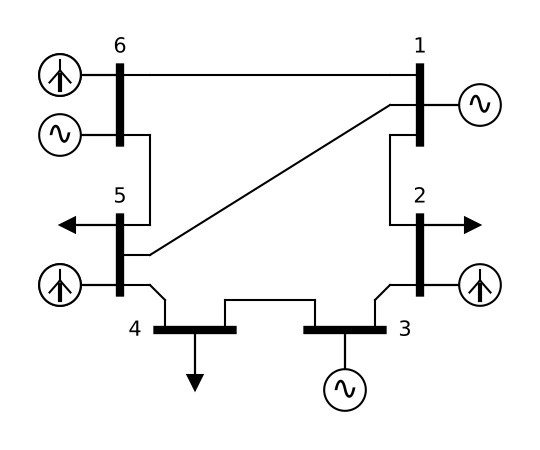
\includegraphics[scale=0.33, trim=0 0 0 0, clip]{6_region_diagram.jpg}
  \end{tabular}
  \begin{tabular}{ l  c}
  Bus & Demand/candidate generation \\ \hline
  1 & baseload, peaking \\
  2 & demand, wind, solar (DE) \\
  3 & baseload, peaking \\
  4 & demand (FR) \\
  5 & demand, wind, solar (UK) \\
  6 & baseload, peaking, wind, solar (ES) \\ \hline
\end{tabular}
  \caption{6-bus model configuration. Demand must be met at buses 2, 5 and 6. Conventional generation (baseload or peaking) may be installed at buses 1, 3 and 6. Wind and solar generation may be installed at buses 2, 5 and 6. Buses 2, 4, 5 and 6 use (demand, wind or solar) time series data from Germany (DE), France (FR), the United Kingdom (UK) and Spain (ES) respectively.}
  \label{fig:model_2:model_diagram}
\end{figure}

\noindent The \texttt{6\_region} model is a more complicated multi-region model. The system's topology is based on the \textit{IEEE 6-bus system}. The available technologies at each bus are based on a renewables-ready version of the 6-bus system introduced by Kamalinia \& Shahidehpour (2010). Figure \ref{fig:model_2:model_diagram} provides a diagram of the model configuration.

The model takes 9 input time series: hourly demand levels, wind capacity factors and solar capacity factor in European countries. In \texttt{plan} mode, the model leads to a generation \& transmission expansion planning problem where the optimal generation \& transmission capacities and hourly generation \& transmission levels for each technology are determined. This problem is either a continuous linear program or a mixed-integer linear program depending on whether the \texttt{baseload\_integer} constraint is activated. In \texttt{operate} mode, the generation \& transmission capacities are fixed and only the hourly generation \& transmission levels are determined. The mathematical details for the model are provided below.

The \texttt{6\_region} model leads to solution nonuniqueness. For example, excess demand in region 2 has no preference between being met from regions 1 or 3. For this reason, the model should only be used for model-wide summary statistics (e.g. the total baseload capacity). If outputs at regional level are desired, regions must de differentiated by having different technologies in each (e.g. by changing the technology prices at regional level). 




\subsection{Planning mode}
\label{sec:appendix:optimisation:model_3}

\noindent \textit{Model inputs}:
\begin{equation}
  \{C_{i}^\text{gen}, \hspace{0.5em} F_{i}^\text{gen}, \hspace{0.5em} d_{r, t}, \hspace{0.5em} w_{r, t} \hspace{0.5em} : \hspace{0.5em} i \in \mathcal{I}; \hspace{0.5em} r \in \mathcal{R}; \hspace{0.5em} t = 1 \ldots T\}.
\label{eq:model_3:inputs}
\end{equation}
\textit{Model outputs:}
\begin{equation}
\{\text{cap}_{i,r}^\text{gen}, \hspace{0.5em} \text{cap}_{r,r'}^\text{tr}, \hspace{0.5em} \text{gen}_{i,r,t}, \hspace{0.5em} \text{tr}_{r,r',t} \hspace{0.5em} : \hspace{0.5em} i \in \mathcal{I}; \hspace{0.5em} r,r' \in \mathcal{R}; \hspace{0.5em} t = 1 \ldots T\}.
\label{eq:model_3:decision_variables}
\end{equation}
The model outputs are determined as the decision variables that solve the following optimisation problem:
\begin{equation}
\min \sum_{r \in \mathcal{R}} \Bigg[ \frac{T}{8760} \Bigg( \underbrace{\sum_{i \in \mathcal{I}} C_i^\text{gen} \text{cap}_{i,r}^\text{gen}}_{\substack{\text{installation cost,} \\ \text{generation capacity}}} + \underbrace{ \frac{1}{2} \sum_{r' \in \mathcal{R}} C_{r,r'}^\text{tr} \text{cap}_{r,r'}^\text{tr} }_{\substack{\text{installation cost,} \\ \text{transmission capacity}}} \Bigg) + \underbrace{ \sum_{i \in \mathcal{I}} \sum_{t=1}^{T} F_i^\text{gen} \text{gen}_{i,r,t}}_\text{generation cost} \Bigg]
\label{eq:model_3:objective}
\end{equation}
\noindent subject to
\begin{align}
\text{cap}_{b,r}^\text{gen} \big\rvert_{r \ne 1, 3, 6} = \text{cap}_{p,r}^\text{gen} \big\rvert_{r \ne 1, 3, 6} = \text{cap}_{w,r}^\text{gen} \big\rvert_{r \ne 2, 5, 6} &= 0 \label{eq:model_3:gen_topology} \\
\text{cap}_{r, r'}^\text{tr} \big\rvert_{\{r, r'\} \ne \{1,2\}, \{1,5\}, \{1,6\}, \{2,3\}, \{3,4\}, \{4,5\}, \{5,6\}} &= 0 \label{eq:model_3:tr_topology} \\
\sum_{i \in \mathcal{I}} \text{gen}_{i,r,t} + \sum_{r'=1}^6 \text{tr}_{r',r,t} = d_{r,t} \quad & \forall \: r, t \label{eq:model_3:demand_met} \\
\text{tr}_{r,r',t} + \text{tr}_{r,'r,t} = 0 \quad & \forall \: r, r', t \label{eq:model_3:tr_balance} \\
\text{gen}_{b,r,t} \le \text{cap}_{b,r}^\text{gen} \quad & \forall \: r, t \label{eq:model_3:gen_le_cap_b} \\
\text{gen}_{p,r,t} \le \text{cap}_{p,r}^\text{gen} \quad & \forall \: r, t \label{eq:model_3:gen_le_cap_p} \\
\text{gen}_{w,r,t} \le \text{cap}_{w,r}^\text{gen} w_{r,t} \quad & \forall \: r, t \label{eq:model_3:gen_le_cap_w} \\
|\text{tr}_{r,r',t}| \le \text{cap}_{r,r'}^\text{tr} \quad & \forall \: r, r', t \label{eq:model_3:tr_le_cap_tr} \\
\text{cap}_{b,r}^\text{gen} \in 3\mathbb{Z} \quad & \forall \: r \label{eq:model_3:integer} \\
|\text{gen}_{b,r,t} - \text{gen}_{b,r,t+1}| \le 0.2 \text{cap}_{b,r}^\text{gen} \quad & \forall \: r, t \label{eq:model_3:ramping} \\
\text{gen}_{u,r,t} = 0 \quad & \forall \: r, t \label{eq:model_3:no_unmet} \\
\text{cap}_{i,r}^\text{gen}, \text{cap}_{r,r'}^\text{tr}, \text{gen}_{i,r,t} \ge 0 \quad & \forall \: i, r, t. \label{eq:model_3:ge_0}
\end{align}
\noindent The $\frac{T}{8760}$ factor ensures the installation and generation costs are scaled correctly in model runs of different simulation lengths. \eqref{eq:model_3:gen_topology}-\eqref{eq:model_3:tr_topology} stipulate the locations of generation technologies and the model's transmission topology. \eqref{eq:model_3:demand_met} and \eqref{eq:model_3:tr_balance} are the demand and power flow balance requirements. \eqref{eq:model_3:gen_le_cap_b}-\eqref{eq:model_3:gen_le_cap_w} ensure generation does not exceed installed capacity (for baseload and peaking) or installed capacity times the wind capacity factor (for wind). \eqref{eq:model_3:tr_le_cap_tr} ensures transmission does not exceed transmission capacity. \eqref{eq:model_3:integer} is the integer constraint (active only if \texttt{baseload\_integer=True}) for baseload capacity, which may only be installed in units of 3GW. \eqref{eq:model_3:ramping} is the ramping constraint (active only if \texttt{baseload\_ramping=True}) for baseload generation, which can ramp up or down at maximally 20\%/hr. \eqref{eq:model_1:no_unmet} (active only if \texttt{allow\_unmet=False}) removes the possibility of unmet demand. \eqref{eq:model_3:ge_0} enforces the nonnegativity of capacity and generation levels.





\subsection{Operation mode}
\label{sec:appendix:optimisation:model_4}
\noindent \textit{Model inputs}:
\begin{equation}
  \{C_{i}^\text{gen}, \hspace{0.5em} F_{i}^\text{gen}, \hspace{0.5em} d_{r, t}, \hspace{0.5em} w_{r, t} \hspace{0.5em}, \text{cap}_{i,r}^\text{gen}, \hspace{0.5em} \text{cap}_{r,r'}^\text{tr}, \hspace{0.5em} : \hspace{0.5em} i \in \mathcal{I}; \hspace{0.5em} r,r' \in \mathcal{R}; \hspace{0.5em} t = 1 \ldots T\}.
\label{eq:model_4:inputs}
\end{equation}
\textit{Model outputs:}
\begin{equation}
\{\text{gen}_{i,r,t}, \hspace{0.5em} \text{tr}_{r,r',t} \hspace{0.5em} : \hspace{0.5em} i \in \mathcal{I}; \hspace{0.5em} r,r' \in \mathcal{R}; \hspace{0.5em} t = 1 \ldots T\}.
\label{eq:model_4:decision_variables}
\end{equation}
The model outputs are determined as the decision variables that solve the following optimisation problem:
\begin{equation}
\min \underbrace{ \sum_{r \in \mathcal{R}} \sum_{i \in \mathcal{I}} \sum_{t=1}^{T} F_i^\text{gen} \text{gen}_{i,r,t}}_\text{generation cost}
\label{eq:model_4:objective}
\end{equation}
\noindent subject to
\begin{align}
\sum_{i \in \mathcal{I}} \text{gen}_{i,r,t} + \sum_{r'=1}^6 \text{tr}_{r',r,t} = d_{r,t} \quad & \forall \: r, t \label{eq:model_4:demand_met} \\
\text{tr}_{r,r',t} + \text{tr}_{r,'r,t} = 0 \quad & \forall \: r, r', t \label{eq:model_4:tr_balance} \\
\text{gen}_{b,r,t} \le \text{cap}_{b,r}^\text{gen} \quad & \forall \: r, t \label{eq:model_4:gen_le_cap_b} \\
\text{gen}_{p,r,t} \le \text{cap}_{p,r}^\text{gen} \quad & \forall \: r, t \label{eq:model_4:gen_le_cap_p} \\
\text{gen}_{w,r,t} \le \text{cap}_{w,r}^\text{gen} w_{r,t} \quad & \forall \: r, t \label{eq:model_4:gen_le_cap_w} \\
|\text{tr}_{r,r',t}| \le \text{cap}_{r,r'}^\text{tr} \quad & \forall \: r, r', t \label{eq:model_4:tr_le_cap_tr} \\
|\text{gen}_{b,r,t} - \text{gen}_{b,r,t+1}| \le 0.2 \text{cap}_{b,r}^\text{gen} \quad & \forall \: r, t \label{eq:model_4:ramping} \\
\text{gen}_{u,r,t} = 0 \quad & \forall \: r, t \label{eq:model_3:no_unmet} \\
\text{gen}_{i,r,t} \ge 0 \quad & \forall \: i, r, t. \label{eq:model_4:ge_0}
\end{align}
\noindent where each constraint has the same meaning as for the planning model.



\section{References}
\label{sec:references}

\noindent HC Bloomfield, DJ Brayshaw, A Charlton-Perez (2019). Characterising the winter meteorological drivers of the European electricity system using targeted circulation types. \textit{Meteorological Applications}. doi:\texttt{10.1002/met.1858}. \\

\noindent S Kamalinia, M Shahidehpour (2010). Generation expansion planning in wind-thermal power systems. \textit{IET Generation, Transmission \& Distribution, 4-8, 940-951}. doi:\texttt{10.1049/iet-gtd.2009.0695}.








\end{document}
